%*******10********20********30********40********50********60********70********80
\chap{Analysis and Design}
Concentrate on explaining the decisions made and the reasons for them.
\section{Web application architecture}

\section{Models design}

\begin{figure}[H]
	\centering
    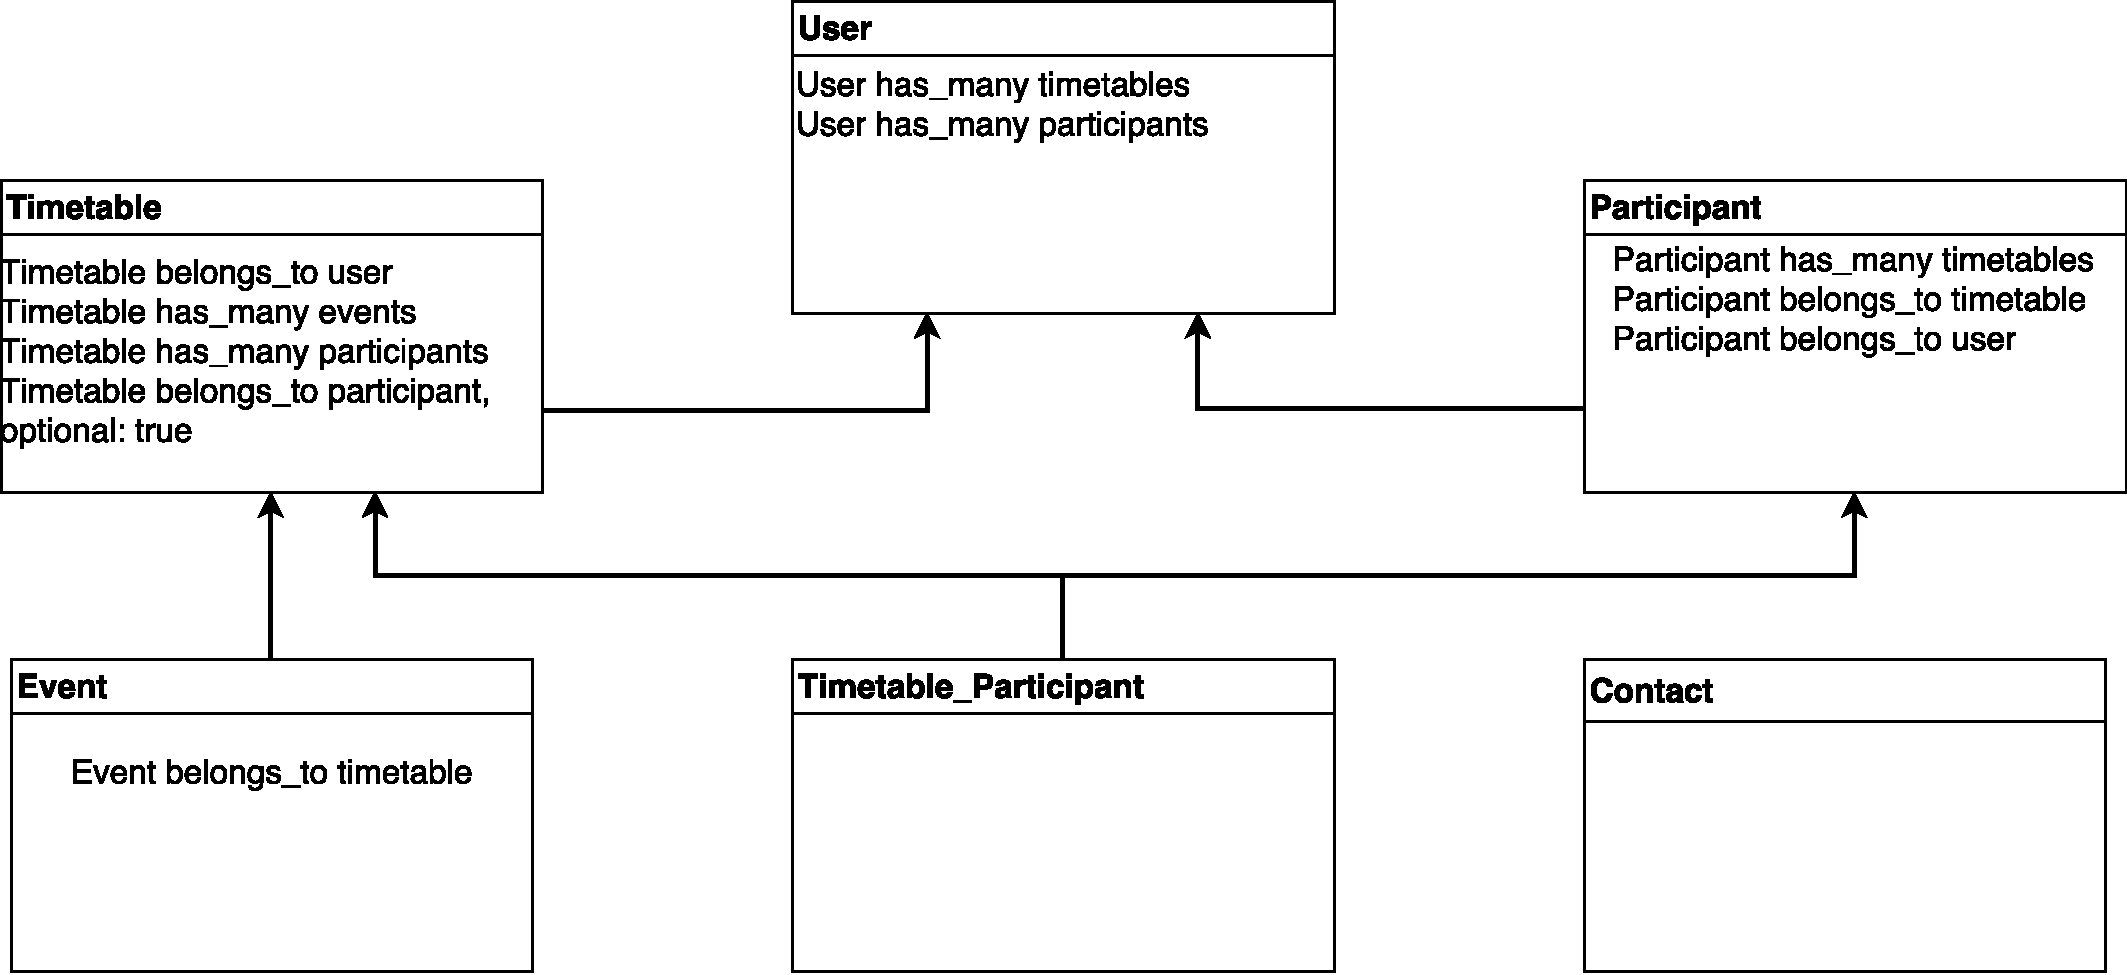
\includegraphics[trim={0 0 0 0},clip,width=1\textwidth]{Files/Models.pdf}
    \caption{Implemented models.}
    \label{fig: Models}
\end{figure}

\subsection{User}
The user model is responsible for keeping track of the application's user information. It is directly related to the timetable and participant models, because each user must be able to own several timetables, as well as participating.\\ 
The rest of the model is set up to ensure that the user information is correct. It validates the user e-mail, uses a Bcrypt function to ensure that all users have passwords, and in turn, hashes the password string so that no plaintext passwords are stored in the database. An added feature also allows the user to upload an avatar (profile picture) for their profile. 

\subsection{Session}
\subsection{Timetable}
The timetable
\subsection{Event}
\subsection{Participant}
\subsection{Contact}
The contact model is a small and simple one, but it contains the necessary parts for a proper e-mail header. 
Whenever a user submits a new contact form, the model validates the fields of the form, as well as one "invisible" field, 
used for catching spam bots. This "spam catcher" works by refusing to submit forms where the field \textit{nickname} 
contains any characters. Since the field being hidden by some CSS code, we know that a human can't see this field, unless they have access to the code, in which case it's most likely a robot of some kind.
 
